\chapter{Operatoren, Observ observablen und die Pauli-Matrizen}

Gute Notation ist keine Dekoration. In einem Fach, das auf abstrakten Vektoren und komplexen Zahlen beruht, gehört eine Notation, mit der wir Symbole verschieben können, ohne sie immer wieder in Worte zu übersetzen, zum Handwerkszeug. Diracs Bra--Ket-Notation ist genau deshalb wertvoll: Sie hält die Geometrie des Zustandsraums sichtbar und erlaubt uns zugleich, mit Komponenten und Matrizen zu rechnen.

Unsere unmittelbare Aufgabe ist mathematischer Natur. Wir führen lineare Operatoren ein, lernen, wie sie auf Bras ebenso wie auf Kets wirken, und grenzen die besondere Klasse der hermiteschen Operatoren ab. Erst dann verbinden wir damit die physikalischen Begriffe \emph{Observable}, \emph{Messergebnis} und \emph{Wahrscheinlichkeit}. So ergeben sich die drei Spinobservablen als Pauli-Matrizen, statt dass man sie uns als auswendig zu lernende Objekte vorsetzt.

\section{Orthonormale Basen und Komponenten}

Die Zustände bilden einen komplexen linearen Vektorraum. Seine Ket-Vektoren lassen sich addieren und mit komplexen Zahlen multiplizieren. Zu jedem Ket \(\ket{A}\) gehört ein Bra \(\bra{A}\), das durch die konjugiert-duale Abbildung entsteht. Eine Basis ist nicht eindeutig festgelegt; sobald man jedoch eine gewählt hat, lässt sich jeder Vektor durch seine Komponenten bezüglich dieser Basis beschreiben.

Sei
\[
\bigl\{\ket{1},\ket{2},\ldots,\ket{N}\bigr\}
\]
eine orthonormale Basis. Orthogonalität und Normierung werden zusammengefasst durch
\begin{equation}
\braket{j}{i}=\delta_{ji}.
\label{eq:orthonormal-basis}
\end{equation}
Hier ist \(\delta_{ji}\) gleich eins, wenn \(j=i\) gilt, und andernfalls null. Die Dimension \(N\) ist die maximale Anzahl paarweise orthogonaler Richtungen im Raum; eine vollständige Orthonormalbasis enthält genau so viele Vektoren.

Entwickeln wir ein beliebiges Ket nach dieser Basis:
\begin{equation}
\ket{A}=\sum_i \alpha_i\ket{i}.
\label{eq:ket-expansion}
\end{equation}
Die Koeffizienten sind nicht rätselhaft. Multiplizieren wir von links mit \(\bra{j}\):
\begin{align}
\braket{j}{A}
 &=\sum_i\alpha_i\braket{j}{i} \\
 &=\sum_i\alpha_i\delta_{ji}
 =\alpha_j.
\end{align}
Damit gilt
\begin{equation}
\alpha_i=\braket{i}{A}.
\label{eq:components-inner-products}
\end{equation}
Die \(i\)-te Komponente ist die Projektion von \(\ket{A}\) auf die \(i\)-te Basisrichtung.

Setzen wir Gleichung~\eqref{eq:components-inner-products} in Gleichung~\eqref{eq:ket-expansion} ein, erhalten wir die besonders nützliche Form
\begin{equation}
\ket{A}=\sum_i\ket{i}\braket{i}{A}.
\label{eq:ket-completeness-action}
\end{equation}
Die Summe hat am Vektor nichts verändert; sie hat ihn lediglich in seine Basisrichtungen zerlegt und anschließend wieder zusammengesetzt. Diesen Schritt werden wir immer wieder verwenden. Man bezeichnet ihn gewöhnlich als \emph{Einfügen eines vollständigen Satzes von Zuständen}, denn
\begin{equation}
\sum_i\ket{i}\bra{i}=\mathbf 1.
\label{eq:resolution-identity}
\end{equation}

Die entsprechende Entwicklung des Bras lautet
\begin{equation}
\bra{A}=\sum_i\braket{A}{i}\bra{i}
       =\sum_i\alpha_i^*\bra{i}.
\label{eq:bra-expansion}
\end{equation}
Die komplexe Konjugation von \(\alpha_i\) ist wesentlich. Beim Übergang von einem Ket zu einem Bra wird jeder numerische Koeffizient komplex konjugiert.

\begin{figure}[htbp]
\centering
\includegraphics[width=0.82\textwidth]{lecture_03_figure_04.png}
\caption{Die beiden definierenden Regeln eines linearen Operators, nach der Wiederholung der Grundlagen zu Basen.}
\lectureframe{00:12:44}
\end{figure}

\section{Lineare Operatoren als Maschinen}

Ein linearer Operator \(M\) ist eine Vorschrift, die ein Eingabe-Ket eindeutig auf ein Ausgabe-Ket abbildet. Ein anschauliches Bild dafür stammt von John Wheeler: eine Maschine mit einem Eingabe- und einem Ausgabeanschluss. Man setzt \(\ket{A}\) ein, dreht das Rad und erhält \(M\ket{A}\). Die Eingabe legt die Ausgabe fest. Umgekehrt muss das nicht gelten: Zwei Eingaben können dieselbe Ausgabe ergeben, und eine inverse Maschine muss nicht existieren.

Das Adjektiv \emph{linear} umfasst zwei Regeln. Für eine komplexe Zahl \(z\) gilt
\begin{align}
M\bigl(z\ket{A}\bigr)&=z\,M\ket{A}, \label{eq:operator-homogeneous}\\
M\bigl(\ket{A}+\ket{B}\bigr)&=M\ket{A}+M\ket{B}.
\label{eq:operator-additive}
\end{align}
Ein Skalar durchläuft die Maschine unverändert, und eine Summe kann Glied für Glied verarbeitet werden. Diese Regeln implizieren auch die Linearität für jede endliche komplexe Linearkombination.

Dieselbe Idee gilt für gewöhnliche dreidimensionale Vektoren. Die Quantenmechanik erfindet lineare Abbildungen nicht. Sie macht sie unverzichtbar, weil der Zustandsraum abstrakt und komplex ist und weil messbare Größen durch eine ausgezeichnete Familie solcher Abbildungen dargestellt werden.

\section{Vom Operator zu seiner Matrix}

Nehmen wir an, die Maschine bilde \(\ket{A}\) auf \(\ket{B}\) ab:
\begin{equation}
M\ket{A}=\ket{B}.
\label{eq:operator-action}
\end{equation}
Wir wählen für Ein- und Ausgabe dieselbe Orthonormalbasis und schreiben
\[
\ket{A}=\sum_j\alpha_j\ket{j},
\qquad
\ket{B}=\sum_i\beta_i\ket{i}.
\]
Um die \(i\)-te Ausgabekomponente zu bestimmen, projizieren wir Gleichung~\eqref{eq:operator-action} mit \(\bra{i}\):
\begin{equation}
\bra{i}M\ket{A}=\braket{i}{B}=\beta_i.
\end{equation}
Nun setzen wir die Entwicklung von \(\ket{A}\) ein:
\begin{align}
\bra{i}M\ket{A}
 &=\sum_j\bra{i}M\ket{j}\braket{j}{A}\\
 &=\sum_j\bra{i}M\ket{j}\alpha_j
 =\beta_i.
\end{align}
Die Zahlen
\begin{equation}
m_{ij}\equiv\bra{i}M\ket{j}
\label{eq:matrix-elements}
\end{equation}
sind die \emph{Matrixelemente} von \(M\) bezüglich der gewählten Basis. Folglich gilt
\begin{equation}
\boxed{\sum_jm_{ij}\alpha_j=\beta_i.}
\label{eq:component-action}
\end{equation}

\begin{figure}[htbp]
\centering
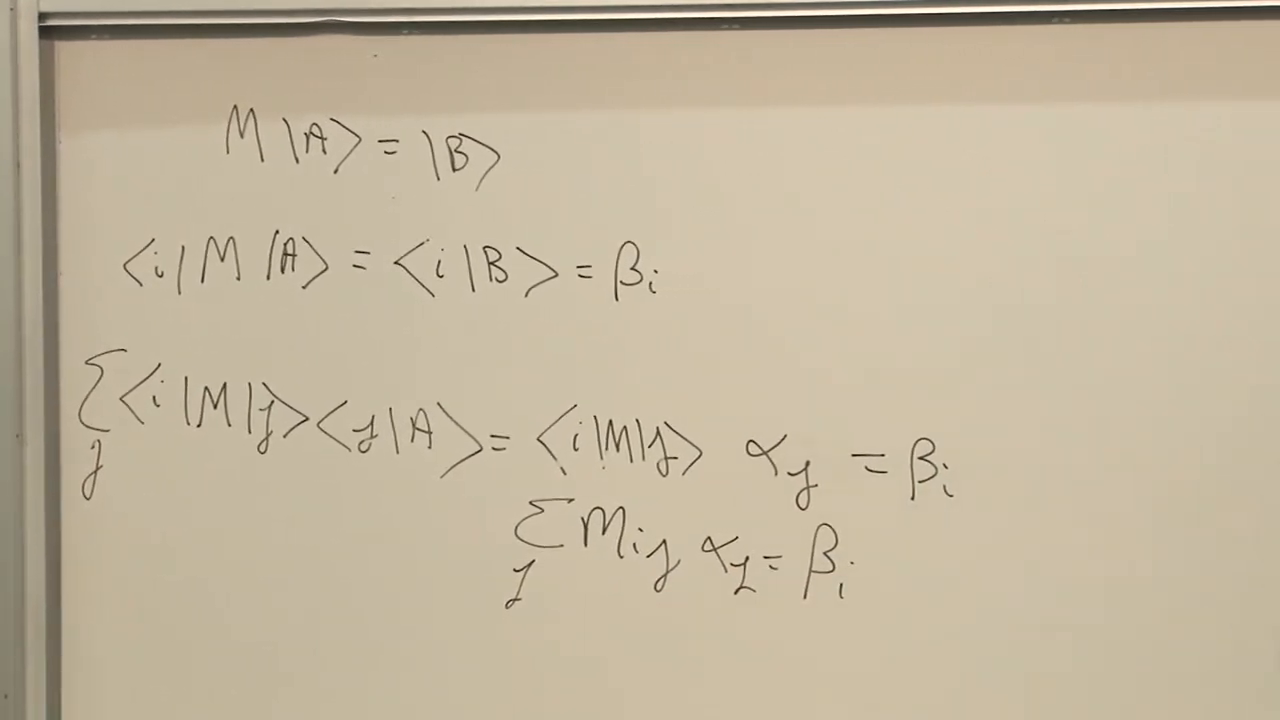
\includegraphics[width=0.84\textwidth]{lecture_03_figure_02.png}
\caption{Die abstrakte Gleichung \(M\ket{A}=\ket{B}\), projiziert und in die Komponentenregel \(\sum_jm_{ij}\alpha_j=\beta_i\) aufgelöst.}
\lectureframe{00:18:30}
\end{figure}

Hat der Raum die Dimension \(N\), bilden die \(N^2\) Zahlen \(m_{ij}\) eine \(N\times N\) quadratische Matrix. Gleichung~\eqref{eq:component-action} lautet genau
\begin{equation}
\begin{pmatrix}
m_{11}&m_{12}&\cdots&m_{1N}\\
m_{21}&m_{22}&\cdots&m_{2N}\\
\vdots&\vdots&\ddots&\vdots\\
m_{N1}&m_{N2}&\cdots&m_{NN}
\end{pmatrix}
\begin{pmatrix}
\alpha_1\\
\alpha_2\\
\vdots\\
\alpha_N
\end{pmatrix}
=
\begin{pmatrix}
\beta_1\\
\beta_2\\
\vdots\\
\beta_N
\end{pmatrix}.
\label{eq:matrix-vector-action}
\end{equation}
Um \(\beta_1\) zu erhalten, multipliziert man die erste Zeile mit der Eingabespalte und addiert die Beiträge; für \(\beta_2\) wiederholt man das mit der zweiten Zeile und so weiter. Die Matrix ist die konkrete Darstellung von Wheelers Maschine.

\begin{figure}[htbp]
\centering
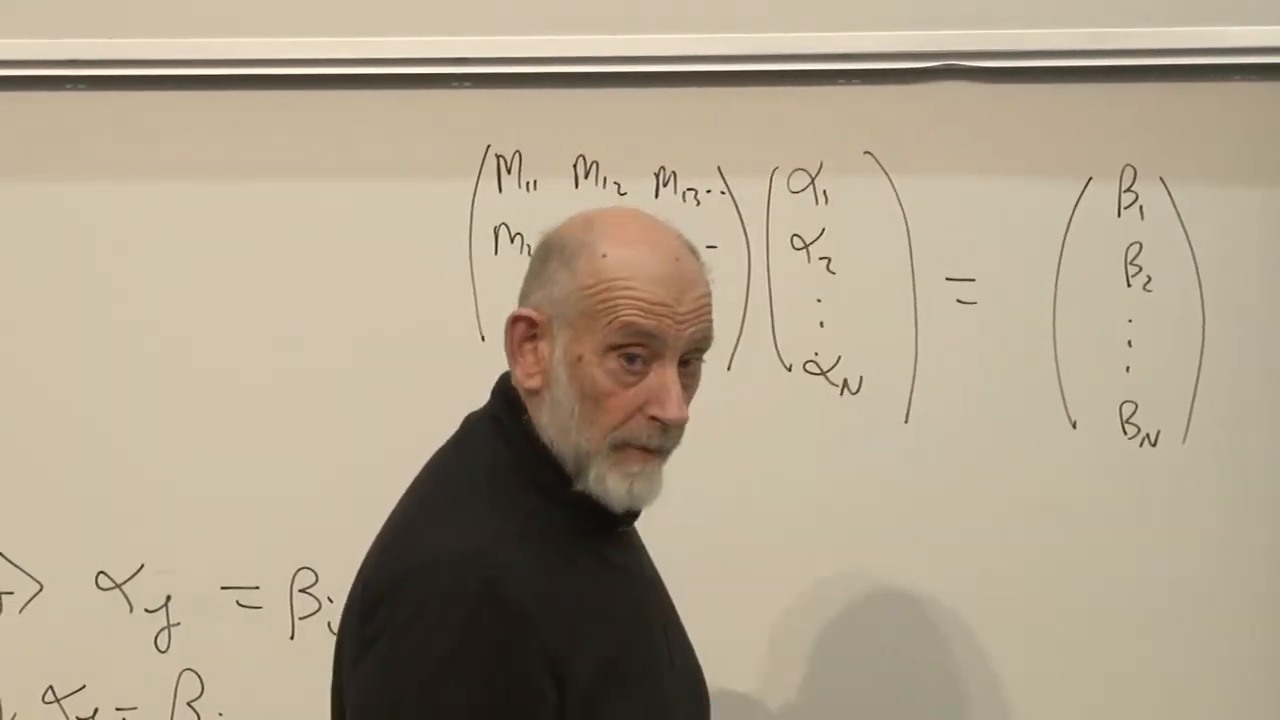
\includegraphics[width=0.84\textwidth]{lecture_03_figure_03.png}
\caption{Dieselbe Operatorwirkung, dargestellt als quadratische Matrix, die mit der Spalte der Eingabekoeffizienten multipliziert wird.}
\lectureframe{00:20:01}
\end{figure}

Wir haben einen Algorithmus gewonnen und etwas von der sichtbaren Geometrie eingebüßt. Die abstrakte Aussage \(M\ket{A}=\ket{B}\) hängt nicht von Koordinaten ab. Die konkreten Einträge \(m_{ij}\), \(\alpha_j\) und \(\beta_i\) hängen dagegen von der gewählten Basis ab. Eine andere Orthonormalbasis verändert alle drei Arrays, lässt aber die zugrunde liegende Abbildung und ihre physikalischen Vorhersagen unverändert.

\begin{classroomqa}
\audiencequestion{Kann die Wahl der Basis darüber entscheiden, ob sich ein Problem lösen lässt?}
\lecturerresponse{Sie kann darüber entscheiden, ob die Lösung leicht zu erkennen ist. Eine geschickt gewählte Basis kann einen Operator diagonal machen und die Rechnung fast unmittelbar erledigen; eine ungünstige Basis kann die Struktur unter unangenehmer Algebra verbergen. Das Ergebnis eines Experiments kann sie nicht ändern. Führen zwei Basen zu unterschiedlichen physikalischen Antworten, ist die Rechnung falsch.}
\end{classroomqa}

\section{Bras, Kets und Antilinearität}

\begin{classroomqa}
\audiencequestion{Kann ein linearer Operator ein Ket in ein Bra oder ein Bra in ein Ket verwandeln?}
\lecturerresponse{Kein gewöhnlicher linearer Operator der gerade definierten Art. Er bildet Kets auf Kets ab, wobei komplexe Skalare unverändert hindurchgehen. Die Abbildung, die Kets und Bras ineinander überführt, komplex konjugiert zugleich ihre Koeffizienten und gehört deshalb zu einer anderen Klasse.}
\end{classroomqa}

Die Multiplikation mit einer festen komplexen Zahl ist ein einfacher linearer Operator. Die komplexe Konjugation ist es nicht. Bezeichnet \(K\) die Konjugation, gilt
\[
K\bigl(z\ket{A}\bigr)=z^*K\ket{A},
\]
nicht aber \(zK\ket{A}\). Eine solche Abbildung heißt \emph{antilinear}. Der Name bedeutet nicht das Gegenteil von linear; er hält fest, dass Skalare komplex konjugiert werden. Ihr tieferer Zusammenhang mit Antiteilchen liegt außerhalb der vorliegenden Diskussion.

Lineare Operatoren lassen sich dennoch auf Bras wirken. Konventionsgemäß schreibt man den Operator rechts:
\begin{equation}
\bra{A}M.
\end{equation}
Die Definition ist so gewählt, dass bei einem Matrixelement keine Unklarheit über die Klammerung entsteht:
\begin{equation}
\bra{A}\bigl(M\ket{B}\bigr)
=
\bigl(\bra{A}M\bigr)\ket{B}
\equiv
\bra{A}M\ket{B}.
\label{eq:bracket-independence}
\end{equation}

Um zu sehen, warum das möglich ist, entwickeln wir beide Vektoren:
\begin{align}
\bra{A}M\ket{B}
 &=\left(\sum_i\alpha_i^*\bra{i}\right)
   M
   \left(\sum_j\beta_j\ket{j}\right)\\
 &=\sum_{ij}\alpha_i^*m_{ij}\beta_j.
\label{eq:matrix-element-double-sum}
\end{align}
Das ist eine gewöhnliche Doppelsumme. Wir können zuerst über \(j\) summieren und \(M\) als auf den Ket-Vektor wirkend auffassen oder zuerst über \(i\) summieren und es als auf den Bra-Vektor wirkend auffassen. Das Ergebnis ist dasselbe. Die Notation ist genau so angelegt, dass sich unnötige Klammern weglassen lassen.

\section{Die Dagger-Operation}

Es gibt eine zweite, davon verschiedene Frage zur Wirkung auf der Bra-Seite. Angenommen,
\[
M\ket{A}=\ket{B}.
\]
Welcher Operator bildet das entsprechende Bra \(\bra{A}\) auf \(\bra{B}\) ab? Im Allgemeinen ist es nicht \(M\) selbst. Wäre \(M\) die Multiplikation mit einer komplexen Zahl \(z\), so lautete die Ket-Gleichung \(\ket{B}=z\ket{A}\), die Bra-Gleichung dagegen \(\bra{B}=z^*\bra{A}\).

Der gesuchte Operator wird mit \(M^\dagger\) bezeichnet, dem \emph{hermiteschen adjungierten Operator} zu \(M\), und ist definiert durch
\begin{equation}
M\ket{A}=\ket{B}
\quad\Longleftrightarrow\quad
\bra{A}M^\dagger=\bra{B}.
\label{eq:dagger-definition}
\end{equation}
Das Dagger ist das Operatoranalogon zur komplexen Konjugation.

Die Matrixregel folgt unmittelbar. Sei
\[
M\ket{i}=\ket{i'}.
\]
Dann gilt
\[
m_{ji}=\bra{j}M\ket{i}=\braket{j}{i'}.
\]
Die adjungierte Bra-Relation lautet \(\bra{i}M^\dagger=\bra{i'}\), also
\[
(m^\dagger)_{ij}
=\bra{i}M^\dagger\ket{j}
=\braket{i'}{j}.
\]
Beim Vertauschen der Reihenfolge eines Skalarprodukts wird dieses komplex konjugiert:
\[
\braket{i'}{j}=\braket{j}{i'}^*.
\]
Daher
\begin{equation}
\boxed{(m^\dagger)_{ij}=m_{ji}^*.}
\label{eq:dagger-matrix-elements}
\end{equation}

\begin{figure}[htbp]
\centering
\includegraphics[width=0.84\textwidth]{lecture_03_figure_05.png}
\caption{Die vervollständigte Tafelrelation für das hermitesche Adjungieren: Indizes vertauschen und komplex konjugieren.}
\lectureframe{00:42:23}
\end{figure}

In Matrixsprache transponieren wir zunächst und komplex konjugieren dann:
\begin{equation}
\begin{pmatrix}
a&b\\
c&d
\end{pmatrix}^{\!\dagger}
=
\begin{pmatrix}
a^*&c^*\\
b^*&d^*
\end{pmatrix}.
\label{eq:dagger-two-by-two}
\end{equation}
Die Transposition spiegelt die Einträge an der Hauptdiagonalen; die Konjugation ersetzt jedes \(i\) durch \(-i\). Zum Beispiel:
\begin{equation}
\begin{pmatrix}
2&6+7i\\
4-i&9+i
\end{pmatrix}^{\!\dagger}
=
\begin{pmatrix}
2&4+i\\
6-7i&9-i
\end{pmatrix}.
\label{eq:dagger-numerical-example}
\end{equation}
Die Diagonaleinträge bleiben an ihrer Position, werden aber komplex konjugiert; die beiden Einträge außerhalb der Diagonale tauschen ihre Plätze und werden ebenfalls komplex konjugiert.

\section{Hermitesche Operatoren}

Eine komplexe Zahl ist genau dann reell, wenn sie ihrer komplexen Konjugierten entspricht. Das Operatoranalogon ergibt sich unmittelbar.

\begin{definition}Ein Operator \(M\) heißt \emph{hermitesch}, wenn
\begin{equation}
M=M^\dagger.
\label{eq:hermitian-definition}
\end{equation}
Äquivalent dazu gilt in jeder Orthonormalbasis
\begin{equation}
m_{ij}=m_{ji}^*.
\label{eq:hermitian-components}
\end{equation}
\end{definition}

Setzen wir \(i=j\) in Gleichung~\eqref{eq:hermitian-components} ein. Dann gilt
\[
m_{ii}=m_{ii}^*,
\]
also ist jeder Diagonaleintrag reell. Abseits der Diagonale treten die Einträge paarweise als Spiegelbilder mit komplexer Konjugation auf. Ist ein Eintrag \(4-i\), so ist sein gespiegelter Partner \(4+i\); ist ein Eintrag die reelle Zahl \(5\), so gilt das auch für seinen Partner.

\begin{figure}[htbp]
\centering
\includegraphics[width=0.78\textwidth]{lecture_03_figure_06.png}
\caption{Ein vollständiges Beispiel für eine hermitesche Matrix: reelle Diagonaleinträge und komplex konjugierte Paare, die an der Diagonalen gespiegelt sind.}
\lectureframe{00:45:43}
\end{figure}

Hermitesche Operatoren sind wichtig, weil sie messbare Größen darstellen werden. Bevor wir diese Zuordnung vornehmen, müssen wir ihre Eigenrichtungen verstehen.

\section{Eigenvektoren und Eigenrichtungen}

Beim ersten Kennenlernen von Eigenvektoren kann dieser Teil im Vergleich zur umgebenden Physik rasch voranschreiten. Die Ideen stammen aus der üblichen linearen Algebra und sind keine neue physikalische Hypothese. Falls sie ungewohnt sind, lohnt es sich, die Definitionen in Ruhe zu wiederholen und dann zur Argumentation zurückzukehren.

Ein allgemeiner Operator ändert die Richtung eines Vektors. Eine Rotation im gewöhnlichen dreidimensionalen Raum etwa dreht fast jeden Vektor von sich selbst weg. Die Rotationsachse ist eine Ausnahme: Ein Vektor entlang dieser Achse behält seine Richtung. Das ist das Modell für einen Eigenvektor.

Eine nichttriviale Rotation einer reellen zweidimensionalen Ebene veranschaulicht die gegenteilige Möglichkeit: Es gibt keine reelle Richtung, die bis auf einen reellen Faktor erhalten bleibt. Ein allgemeiner Operator auf einem eingeschränkten reellen Raum muss also keinen reellen Eigenvektor besitzen. Die hermiteschen Operatoren auf den komplexen Zustandsräumen der Quantenmechanik haben deutlich stärkere Eigenschaften.

Ein Eigenvektor von \(M\) erfüllt
\begin{equation}
M\ket{i}=\lambda_i\ket{i}.
\label{eq:eigenvalue-equation}
\end{equation}
Die Zahl \(\lambda_i\) ist der zugehörige Eigenwert. Der Eigenvektor gehört zum Operator; man spricht nicht von einem Eigenvektor, ohne die Abbildung anzugeben, deren Richtung er erhält.

Seine Länge und Phase sind durch Gleichung~\eqref{eq:eigenvalue-equation} nicht festgelegt. Für jede von null verschiedene komplexe Zahl \(z\) gilt
\[
M\bigl(z\ket{i}\bigr)
=zM\ket{i}
=\lambda_i\bigl(z\ket{i}\bigr).
\]
Daher ist es genauer, von einer \emph{Eigenrichtung} zu sprechen: Jedes von null verschiedene Vielfache von \(\ket{i}\) beschreibt dieselbe Richtung und hat denselben Eigenwert. Üblicherweise wählen wir einen normierten Repräsentanten.

Der zentrale spektrale Satz lautet: Ein hermitescher Operator auf einem \(N\)-dimensionalen komplexen Vektorraum besitzt eine vollständige Orthonormalbasis aus \(N\) Eigenvektoren. Zwei Teile dieser Aussage lassen sich mit sehr wenig Algebra erkennen.

\subsection{Hermitesche Eigenwerte sind reell}

Nehmen wir an, \(M=M^\dagger\) gelte, und
\[
M\ket{i}=\lambda_i\ket{i}.
\]
Bilden wir das hermitesch Adjungierte der ganzen Gleichung:
\begin{equation}
\bra{i}M^\dagger=\lambda_i^*\bra{i}.
\label{eq:eigen-bra-equation}
\end{equation}
Da \(M^\dagger=M\) gilt, multiplizieren wir die Ket-Gleichung mit \(\bra{i}\) und die Bra-Gleichung mit \(\ket{i}\):
\begin{align}
\bra{i}M\ket{i}&=\lambda_i\braket{i}{i},\\
\bra{i}M\ket{i}&=\lambda_i^*\braket{i}{i}.
\end{align}
Derselbe von null verschiedene Normfaktor multipliziert beide Zahlen, also gilt
\begin{equation}
\lambda_i=\lambda_i^*.
\end{equation}
Jeder Eigenwert eines hermiteschen Operators ist reell. Das ist ein erster Hinweis darauf, dass ein solcher Operator die reelle Zahl darstellen kann, die ein Messgerät anzeigt.

\subsection{Verschiedene Eigenwerte ergeben orthogonale Eigenvektoren}

Seien
\[
M\ket{i}=\lambda_i\ket{i},
\qquad
M\ket{j}=\lambda_j\ket{j},
\]
wobei \(M\) hermitesch ist. Adjungieren wir die zweite Gleichung. Dass ihr Eigenwert reell ist, wissen wir bereits:
\[
\bra{j}M=\lambda_j\bra{j}.
\]
Nun multiplizieren wir die erste Gleichung mit \(\bra{j}\) und die Bra-Gleichung mit \(\ket{i}\):
\begin{align}
\bra{j}M\ket{i}&=\lambda_i\braket{j}{i},\\
\bra{j}M\ket{i}&=\lambda_j\braket{j}{i}.
\end{align}
Subtraktion ergibt
\begin{equation}
\boxed{(\lambda_i-\lambda_j)\braket{j}{i}=0.}
\label{eq:hermitian-orthogonality}
\end{equation}
Wenn \(\lambda_i\ne\lambda_j\) gilt, dann folgt
\[
\braket{j}{i}=0.
\]
Die Eigenrichtungen sind orthogonal.

\begin{figure}[htbp]
\centering
\includegraphics[width=0.82\textwidth]{lecture_03_figure_07.png}
\caption{Die entscheidende Zeile des Orthogonalitätsbeweises: Verschiedene Eigenwerte erzwingen, dass das Skalarprodukt verschwindet.}
\lectureframe{00:59:00}
\end{figure}

Sind zwei Eigenwerte gleich, legt Gleichung~\eqref{eq:hermitian-orthogonality} innerhalb des zugehörigen entarteten Eigenraums keine Bedingung fest. Dort können wir eine Orthonormalbasis wählen. Zusammen mit den übrigen Eigenrichtungen bilden diese Vektoren die vom Spektralsatz zugesagte vollständige Orthonormaleigenbasis.

Orthogonalität hat auch eine physikalische Deutung. Zwei orthogonale Zustände lassen sich durch eine geeignete Messung eindeutig unterscheiden. Eigenzustände mit verschiedenen Eigenwerten müssen unterscheidbar sein, weil das Messgerät für sie unterschiedliche reelle Zahlen anzeigt. Die Algebra und die operationale Bedeutung weisen bereits auf dieselbe Zuordnung hin.

\section{Die Messpostulate}

Nun haben wir genügend Formalismus, um die grundlegenden Zuordnungen der Quantenmechanik zu formulieren. Beim ersten Kennenlernen mögen sie fremdartig klingen. Ihre Bedeutung wird erst durch die Anwendung konkret. Formulieren wir sie also klar und kehren wir anschließend sofort zum Spinexperiment zurück.

Eine einzelne Messung liefert eine reelle Zahl. Zwei miteinander verträgliche reelle Messwerte lassen sich zwar zu einer komplexen Zahl zusammenfassen, doch enthält dieses Paket weiterhin zwei Messungen. Das elementare Ergebnis eines einzelnen Detektors ist reell. Hermitesche Operatoren sind daher die naheliegenden Kandidaten: Ihre Eigenwerte sind reell, und ihre Eigenvektoren bilden eine vollständige Orthonormalbasis.

\begin{enumerate}
\item Eine messbare Größe, auch \emph{Observable} genannt, wird durch einen hermiteschen Operator \(M\) dargestellt.
\item Die möglichen Ergebnisse einer Messung von \(M\) sind seine Eigenwerte \(\lambda_i\).
\item Ein Zustand, in dem \(M\) den bestimmten Wert \(\lambda_i\) hat, ist ein Eigenzustand \(\ket{i}\) mit
\[
M\ket{i}=\lambda_i\ket{i}.
\]
\item Befindet sich das System in einem allgemeinen normierten Zustand \(\ket{A}\), so beträgt die Wahrscheinlichkeit, \(\lambda_i\) zu erhalten,
\begin{equation}
P(\lambda_i\mid A)
=\left|\braket{i}{A}\right|^2
=\braket{i}{A}\braket{A}{i}.
\label{eq:born-rule}
\end{equation}
\end{enumerate}

Diese Liste ist ein zweckmäßiger Ausgangspunkt, aber nicht notwendigerweise ein minimales unabhängiges Axiomensystem; in einer sparsameren Formulierung lassen sich manche Aussagen aus anderen herleiten. Wenn wir die Zuordnungen getrennt aufführen, sind ihre physikalischen Rollen leichter zu erkennen.

Die komplexe Zahl \(\braket{i}{A}\) ist eine \emph{Wahrscheinlichkeitsamplitude}, keine Wahrscheinlichkeit. Ihre Multiplikation mit der komplex Konjugierten ergibt eine reelle, nichtnegative Zahl. Für eine Spin-Komponente gibt es nur zwei Spektralwerte, \(+1\) und \(-1\); eine allgemeinere Observable kann viele Eigenwerte haben.

\begin{figure}[htbp]
\centering
\includegraphics[width=0.82\textwidth]{lecture_03_figure_08.png}
\caption{Die Tafel verknüpft Zustände mit eindeutigem Messergebnis mit Eigenvektoren und die Wahrscheinlichkeit für \(\lambda_i\) mit dem Quadrat der Projektion auf \(\ket{i}\).}
\lectureframe{01:11:29}
\end{figure}

\begin{classroomqa}
\audiencequestion{Was steht in der Wahrscheinlichkeitsregel genau neben \(P\)?}
\lecturerresponse{Es ist \(\lambda_i\): \(P(\lambda_i\mid A)\) bezeichnet die Wahrscheinlichkeit, dass eine Messung von \(M\) bei einem in \(\ket{A}\) präparierten System den bestimmten Eigenwert \(\lambda_i\) ergibt. Die rechte Seite ist das Betragsquadrat der Projektion auf den zugehörigen Eigenvektor.}
\end{classroomqa}

\subsection{Normierung und Vollständigkeit}

Die Wahrscheinlichkeiten aller paarweise ausschließlichen Ergebnisse müssen sich zu eins summieren:
\begin{equation}
\sum_i\left|\braket{i}{A}\right|^2=1.
\label{eq:probability-normalization}
\end{equation}
Setzen wir die vollständige Eigenbasis ein:
\begin{align}
\sum_i\left|\braket{i}{A}\right|^2
 &=\sum_i\braket{A}{i}\braket{i}{A}\\
 &=\bra{A}\left(\sum_i\ket{i}\bra{i}\right)\ket{A}\\
 &=\braket{A}{A}.
\end{align}
Damit muss ein zulässiger Zustandsvektor normiert sein:
\begin{equation}
\braket{A}{A}=1.
\label{eq:state-normalization}
\end{equation}
Für \(\ket{A}=\sum_i\alpha_i\ket{i}\) lautet dieselbe Bedingung
\begin{equation}
\sum_i\alpha_i^*\alpha_i=1.
\label{eq:component-normalization}
\end{equation}
Dies ist eine reelle Nebenbedingung für die komplexen Komponenten.

\begin{classroomqa}
\audiencequestion{Muss jede Wahrscheinlichkeit positiv sein?}
\lecturerresponse{Ja. Jede Wahrscheinlichkeit ist eine Zahl multipliziert mit ihrer eigenen komplex Konjugierten und daher nichtnegativ. Durch die Normierung summieren sich alle diese Zahlen zu eins.}
\end{classroomqa}

Es gibt noch eine weitere Redundanz. Multiplizieren wir jede Komponente mit derselben Phase,
\begin{equation}
\ket{A}\longmapsto e^{i\theta}\ket{A},
\label{eq:l3-global-phase}
\end{equation}
so wird jede Amplitude mit \(e^{i\theta}\) multipliziert, während alle Betragsquadrate unverändert bleiben. Diese gemeinsame Phase ist durch keine Messung nachweisbar. Relative Phasen zwischen den Komponenten bleiben physikalisch relevant; nur eine Phase, die den gesamten Zustand multipliziert, ist redundant.

Zwei reelle Parameter eines beliebigen komplexen Vektors legen den physikalischen Zustand also nicht fest: Seine Größe ist durch die Normierung bestimmt, und seine Gesamtphase ist unbeobachtbar. Dieselbe Parameterzählung wie für einen einzelnen Spin ergibt sich nun aus der allgemeinen Wahrscheinlichkeitsregel.

\subsection{Eine Messung präpariert zugleich den Zustand}

Ein weiteres Postulat lässt sich leichter aussprechen, als auf einer kurzen Tafelzeile zusammenfassen. Ergibt eine Messung \(\lambda_i\), befindet sich das System unmittelbar danach im zugehörigen Eigenzustand \(\ket{i}\). Das Messgerät zeichnet also nicht nur ein Ergebnis auf, sondern präpariert auch einen Zustand, in dem eine Wiederholung derselben Messung genau dieses Ergebnis liefert.

\begin{classroomqa}
\audiencequestion{Könnte man die Aussage über Messung und Präparation noch einmal wiederholen?}
\lecturerresponse{Vor der Messung können mehrere Eigenwerte mit den in Gleichung~\eqref{eq:born-rule} angegebenen Wahrscheinlichkeiten auftreten. Sobald das Messgerät tatsächlich \(\lambda_i\) anzeigt, befindet sich das System im Eigenzustand zum Eigenwert \(\lambda_i\). Eine unmittelbar anschließende zweite Messung derselben Observable ergibt deshalb denselben Wert.}
\end{classroomqa}

\begin{classroomqa}
\audiencequestion{Sagen diese Prinzipien bereits, wie sich der Zustand mit der Zeit entwickelt?}
\lecturerresponse{Noch nicht. Wir haben festgelegt, was ein Zustand ist, wie Observablen dargestellt werden und was eine Messung bewirkt. Das Gesetz der zeitlichen Entwicklung ist eine zusätzliche Struktur und wird später eingeführt. Das entspricht dem Vorgehen, zunächst den klassischen Phasenraum zu definieren, bevor man die Bewegungsgleichungen aufstellt.}
\end{classroomqa}

\begin{classroomqa}
\audiencequestion{Früher trat beim mittleren Spin entlang einer geneigten Achse \(\cos\theta\) auf. Sollte die neue Regel mit quadrierten Amplituden daraus \(\cos^2\theta\) machen?}
\lecturerresponse{Wahrscheinlichkeit und Mittelwert sind verschiedene Größen. Der Mittelwert kombiniert die Wahrscheinlichkeiten der Ergebnisse \(+1\) und \(-1\) mit ihren Vorzeichen. Sobald der Spinor für eine beliebige Richtung konstruiert ist, liefern die quadrierten Amplituden wieder den zuvor erhaltenen Kosinus-Mittelwert. Diese Rechnung ist die nächste Anwendung; man sollte sie nicht durch bloßes Ändern der alten Formel erraten.}
\end{classroomqa}

\section{Spin als erste Anwendung}

Die drei messbaren Spin-Komponenten werden durch hermitesche Operatoren dargestellt:
\[
\sigma_x,\qquad \sigma_y,\qquad \sigma_z.
\]
Die Analysatorexperimente haben bereits ihre möglichen Werte und die Zustände mit eindeutigem Wert geliefert:
\[
\begin{array}{c|c|c}
\text{observable}&\text{eigenvalue }+1&\text{eigenvalue }-1\\ \hline
\sigma_z&\ket{u}&\ket{d}\\
\sigma_x&\ket{r}&\ket{l}\\
\sigma_y&\ket{\mathrm{in}}&\ket{\mathrm{out}}
\end{array}
\]
Diese Angaben reichen aus, um die Operatoren als Matrizen zu rekonstruieren.

\subsection{Die z-Komponente in ihrer Eigenbasis}

Wir wählen die Up--Down-Basis. Ein bestimmter \(z\)-Spin bedeutet
\begin{equation}
\sigma_z\ket{u}=+\ket{u},
\qquad
\sigma_z\ket{d}=-\ket{d}.
\label{eq:sigma-z-eigenvectors}
\end{equation}
Die beiden Eigenwerte sind verschieden, also folgt aus der Hermitizität \(\braket{u}{d}=0\).

Berechnen wir die vier Matrixelemente:
\begin{align}
\bra{u}\sigma_z\ket{u}&=+1,&
\bra{u}\sigma_z\ket{d}&=-\braket{u}{d}=0,\\
\bra{d}\sigma_z\ket{u}&=\braket{d}{u}=0,&
\bra{d}\sigma_z\ket{d}&=-1.
\end{align}
Daher gilt
\begin{equation}
\boxed{
\sigma_z=
\begin{pmatrix}
1&0\\
0&-1
\end{pmatrix}_{\{u,d\}}.}
\label{eq:sigma-z}
\end{equation}
Die Koordinatenspalten lauten
\[
\ket{u}\widehat{=}\begin{pmatrix}1\\0\end{pmatrix},
\qquad
\ket{d}\widehat{=}\begin{pmatrix}0\\1\end{pmatrix}.
\]
Die Multiplikation mit Gleichung~\eqref{eq:sigma-z} lässt die erste Spalte unverändert und versieht die zweite mit einem Minuszeichen, genau wie es die Eigenwertgleichungen verlangen.

\begin{figure}[htbp]
\centering
\includegraphics[width=0.82\textwidth]{lecture_03_figure_09.png}
\caption{Die Eigenwertgleichungen zu \(\sigma_z\) und die daraus folgende Diagonalmatrix in der Up--Down-Basis.}
\lectureframe{01:26:56}
\end{figure}

\subsection{Die x-Komponente ohne Basiswechsel}

In der Rechts--Links-Basis hätte \(\sigma_x\) dieselbe Diagonalform. Das wäre einfach, aber wenig aufschlussreich. Wir behalten die Up--Down-Basis und verwenden
\begin{equation}
\sigma_x\ket{r}=+\ket{r},
\qquad
\sigma_x\ket{l}=-\ket{l}.
\label{eq:sigma-x-eigenvectors}
\end{equation}
Die beiden Basen hängen wie folgt zusammen:
\begin{align}
\ket{r}&=\frac{\ket{u}+\ket{d}}{\sqrt2},&
\ket{l}&=\frac{\ket{u}-\ket{d}}{\sqrt2},\\
\ket{u}&=\frac{\ket{r}+\ket{l}}{\sqrt2},&
\ket{d}&=\frac{\ket{r}-\ket{l}}{\sqrt2}.
\label{eq:x-z-basis-relations}
\end{align}

Beginnen wir mit dem oberen Diagonaleintrag:
\begin{align}
\bra{u}\sigma_x\ket{u}
 &=\frac12(\bra{r}+\bra{l})\sigma_x(\ket{r}+\ket{l})\\
 &=\frac12(\bra{r}+\bra{l})(\ket{r}-\ket{l})\\
 &=0.
\end{align}
Die Rechts- und Links-Zustände sind orthonormal, daher heben sich die beiden Diagonalbeiträge auf und die Kreuzterme verschwinden. Dieselbe Rechnung mit \(\ket{d}\) ergibt
\[
\bra{d}\sigma_x\ket{d}=0.
\]
An dieser Stelle bedeuten zwei Nullen nicht, dass der Operator verschwindet; sie zeigen, dass wir die Einträge außerhalb der Diagonalen betrachten müssen.

Für den Eintrag oben rechts gilt
\begin{align}
\bra{u}\sigma_x\ket{d}
 &=\frac12(\bra{r}+\bra{l})\sigma_x(\ket{r}-\ket{l})\\
 &=\frac12(\bra{r}+\bra{l})(\ket{r}+\ket{l})\\
 &=1.
\end{align}
Aus der Hermitizität oder durch direkte Wiederholung der Rechnung folgt
\[
\bra{d}\sigma_x\ket{u}=1.
\]
Damit erhalten wir
\begin{equation}
\boxed{
\sigma_x=
\begin{pmatrix}
0&1\\
1&0
\end{pmatrix}_{\{u,d\}}.}
\label{eq:sigma-x}
\end{equation}
Derselbe abstrakte Operator ist in seiner eigenen Eigenbasis diagonal und in der \(z\)-Basis nichtdiagonal. Das ist ein konkretes Beispiel für Basisabhängigkeit ohne physikalische Mehrdeutigkeit.

\subsection{Die y-Komponente und die relative Phase}

Wir wählen die normierte Ein--Aus-Konvention
\begin{equation}
\ket{\mathrm{in}}=\frac{\ket{u}+i\ket{d}}{\sqrt2},
\qquad
\ket{\mathrm{out}}=\frac{\ket{u}-i\ket{d}}{\sqrt2},
\label{eq:l3-in-out-states}
\end{equation}
mit
\[
\sigma_y\ket{\mathrm{in}}=+\ket{\mathrm{in}},
\qquad
\sigma_y\ket{\mathrm{out}}=-\ket{\mathrm{out}}.
\]
Eine Vertauschung der Bezeichnungen oder eine Umkehrung der \(y\)-Achse ändert die Vorzeichenkonvention, nicht die zugrunde liegende Konstruktion. Mit Gleichung~\eqref{eq:l3-in-out-states} ist die einzige hermitesche Matrix mit diesen Eigenvektoren und Eigenwerten
\begin{equation}
\boxed{
\sigma_y=
\begin{pmatrix}
0&-i\\
i&0
\end{pmatrix}_{\{u,d\}}.}
\label{eq:sigma-y}
\end{equation}
Sie lässt sich leicht überprüfen, statt sie erneut herzuleiten:
\begin{align}
\begin{pmatrix}0&-i\\i&0\end{pmatrix}
\frac1{\sqrt2}\begin{pmatrix}1\\i\end{pmatrix}
&=\frac1{\sqrt2}\begin{pmatrix}1\\i\end{pmatrix},\\
\begin{pmatrix}0&-i\\i&0\end{pmatrix}
\frac1{\sqrt2}\begin{pmatrix}1\\-i\end{pmatrix}
&=-\frac1{\sqrt2}\begin{pmatrix}1\\-i\end{pmatrix}.
\end{align}
Die Faktoren \(1/\sqrt2\) normieren die Eigenvektoren, beeinflussen ihre Eigenrichtungen aber nicht.

\begin{figure}[htbp]
\centering
\includegraphics[width=0.82\textwidth]{lecture_03_figure_10.png}
\caption{Der vervollständigte Satz der Pauli-Matrizen in der Up--Down-Basis.}
\lectureframe{01:38:11}
\end{figure}

\begin{classroomqa}
\audiencequestion{Sollte man ein Vorzeichen in den Ein--Aus-Vektoren ändern, damit sie orthogonal sind?}
\lecturerresponse{Nein. Der fehlende Schritt ist die komplexe Konjugation, wenn man den Ket in ein Bra umwandelt:
\[
\bra{\mathrm{in}}=\frac{\bra{u}-i\bra{d}}{\sqrt2}.
\]
Daher
\[
\begin{aligned}
\braket{\mathrm{in}}{\mathrm{out}}
&=\frac12(\bra{u}-i\bra{d})
  (\ket{u}-i\ket{d})\\
&=\frac12\bigl(1+(-i)(-i)\bigr)\\
&=0.
\end{aligned}
\]
Das Vergessen dieser Konjugation ist genau der häufige Fehler, den die Bra--Ket-Notation sichtbar machen soll.}
\end{classroomqa}

Wir haben erhalten:
\begin{equation}
\begin{aligned}
\sigma_x&=\begin{pmatrix}0&1\\1&0\end{pmatrix},\\[0.4em]
\sigma_y&=\begin{pmatrix}0&-i\\i&0\end{pmatrix},\\[0.4em]
\sigma_z&=\begin{pmatrix}1&0\\0&-1\end{pmatrix}.
\end{aligned}
\label{eq:pauli-triple}
\end{equation}
Sie sind hermitesch, haben die Eigenwerte \(\pm1\) und besitzen genau die Eigenvektoren mit bestimmtem Spin, die von den Analysatorexperimenten verlangt werden.

Damit ist das nächste Problem klar gestellt. Gegeben sei ein Spin, der entlang einer beliebigen Richtung präpariert wurde. Konstruiere den zugehörigen Zustand und berechne mithilfe quadrierter Amplituden die Wahrscheinlichkeiten für \(\sigma_z=+1\) und \(\sigma_z=-1\). Der Formalismus enthält bereits alle nötigen Informationen; diese Rechnung durchzuführen ist der folgerichtige nächste Schritt.
